% Membuat gambar contoh bertema alat/sistem (data dan nama komponen fiktif untuk ilustrasi format).
% Satu halaman per gambar, lalu diubah ke PNG: contoh-sistem.png, contoh-esp32.png, contoh-kerangka.png,
% contoh-alur.png, contoh-rangkaian.png, contoh-prototipe.png  (lihat contoh-alat.sh di folder ini)
\documentclass[multi=tikzpicture,border=4pt]{standalone}
\usepackage{fontspec}
\IfFontExistsTF{Times New Roman}{\setmainfont{Times New Roman}}{\setmainfont{TeX Gyre Termes}}
\usepackage{tikz}
\usetikzlibrary{shapes.geometric,arrows.meta,positioning,calc,decorations.pathreplacing}
\tikzset{
  kotak/.style={draw,thick,rectangle,rounded corners=2pt,minimum width=2.6cm,minimum height=1.1cm,align=center,font=\small,fill=white},
  term/.style={draw,thick,rectangle,rounded corners=9pt,minimum width=2.6cm,minimum height=0.8cm,font=\small,fill=white},
  proses/.style={draw,thick,rectangle,minimum width=6.4cm,text width=6.0cm,minimum height=0.9cm,align=center,font=\small,fill=white},
  io/.style={draw,thick,trapezium,trapezium left angle=70,trapezium right angle=110,minimum width=6.4cm,text width=5.0cm,minimum height=0.9cm,align=center,font=\small,fill=white},
  putus/.style={draw,thick,diamond,aspect=2.4,align=center,font=\small,inner sep=1pt,fill=white},
  panah/.style={-{Stealth[length=2.4mm]},thick},
  pin/.style={font=\scriptsize,inner sep=1pt}
}
\begin{document}
% ---------- 1. Gambaran umum sistem ----------
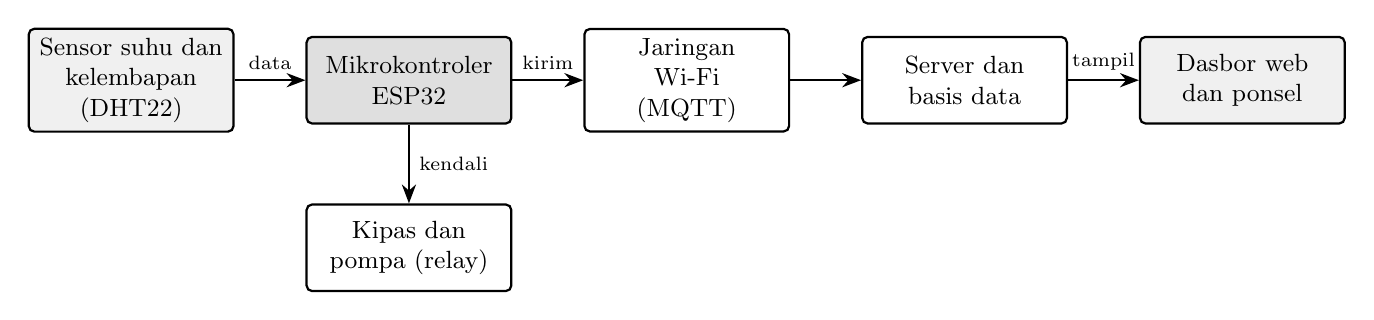
\begin{tikzpicture}[node distance=0.9cm]
\node[kotak,fill=gray!12] (s) {Sensor suhu dan\\ kelembapan\\ (DHT22)};
\node[kotak,right=of s,fill=gray!25] (m) {Mikrokontroler\\ ESP32};
\node[kotak,right=of m] (w) {Jaringan\\ Wi-Fi\\ (MQTT)};
\node[kotak,right=of w] (v) {Server dan\\ basis data};
\node[kotak,right=of v,fill=gray!12] (d) {Dasbor web\\ dan ponsel};
\node[kotak,below=1.0cm of m] (a) {Kipas dan\\ pompa (relay)};
\draw[panah] (s) -- node[above,font=\scriptsize]{data} (m);
\draw[panah] (m) -- node[above,font=\scriptsize]{kirim} (w);
\draw[panah] (w) -- (v);
\draw[panah] (v) -- node[above,font=\scriptsize]{tampil} (d);
\draw[panah] (m) -- node[right,font=\scriptsize]{kendali} (a);
\end{tikzpicture}
% ---------- 2. Papan mikrokontroler (sketsa alat) ----------
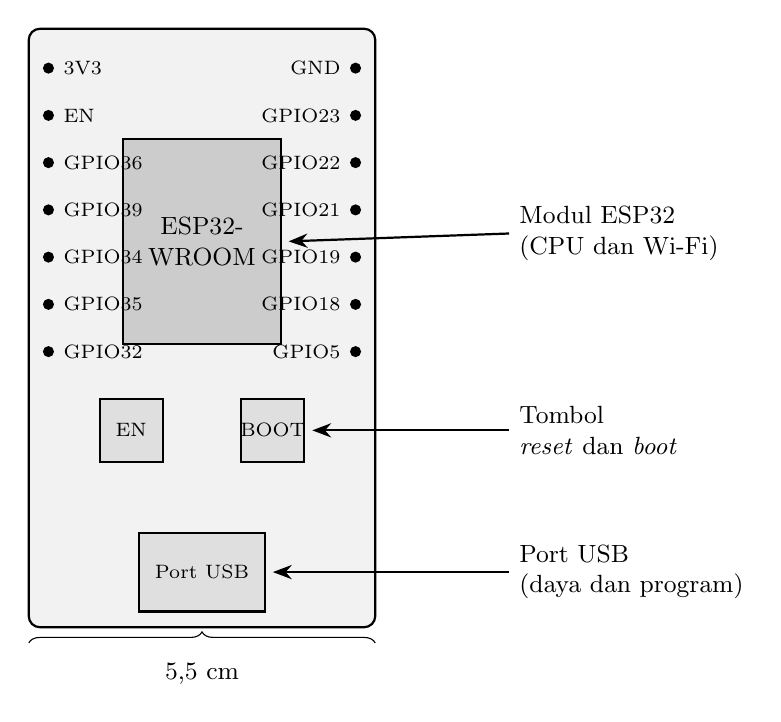
\begin{tikzpicture}
\draw[thick,rounded corners=4pt,fill=gray!10] (0,0) rectangle (4.4,7.6);
\draw[thick,fill=gray!40] (1.2,3.6) rectangle (3.2,6.2); \node[font=\small,align=center] at (2.2,4.9) {ESP32-\\ WROOM};
\draw[thick,fill=gray!25] (1.4,0.2) rectangle (3.0,1.2); \node[font=\scriptsize] at (2.2,0.7) {Port USB};
\draw[thick,fill=gray!25] (0.9,2.1) rectangle (1.7,2.9); \node[font=\scriptsize] at (1.3,2.5) {EN};
\draw[thick,fill=gray!25] (2.7,2.1) rectangle (3.5,2.9); \node[font=\scriptsize] at (3.1,2.5) {BOOT};
\foreach \y/\l/\r in {7.1/3V3/GND,6.5/EN/GPIO23,5.9/GPIO36/GPIO22,5.3/GPIO39/GPIO21,4.7/GPIO34/GPIO19,4.1/GPIO35/GPIO18,3.5/GPIO32/GPIO5}{
  \fill (0.25,\y) circle (2pt); \fill (4.15,\y) circle (2pt);
  \node[pin,anchor=west] at (0.4,\y) {\l}; \node[pin,anchor=east] at (4.0,\y) {\r};}
\draw[panah] (6.1,5.0) node[right,font=\small,align=left]{Modul ESP32\\ (CPU dan Wi-Fi)} -- (3.3,4.9);
\draw[panah] (6.1,0.7) node[right,font=\small,align=left]{Port USB\\ (daya dan program)} -- (3.1,0.7);
\draw[panah] (6.1,2.5) node[right,font=\small,align=left]{Tombol\\ \textit{reset} dan \textit{boot}} -- (3.6,2.5);
\draw[decorate,decoration={brace,amplitude=4pt}] (0,-0.2) -- node[below=4pt,font=\small]{5,5 cm} (4.4,-0.2);
\end{tikzpicture}
% ---------- 3. Kerangka pikir ----------
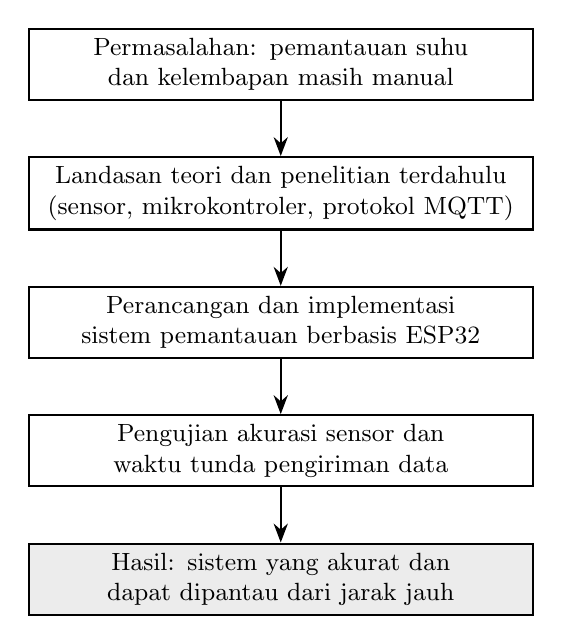
\begin{tikzpicture}[node distance=0.7cm]
\node[proses] (a) {Permasalahan: pemantauan suhu\\ dan kelembapan masih manual};
\node[proses,below=of a] (b) {Landasan teori dan penelitian terdahulu\\ (sensor, mikrokontroler, protokol MQTT)};
\node[proses,below=of b] (c) {Perancangan dan implementasi\\ sistem pemantauan berbasis ESP32};
\node[proses,below=of c] (d) {Pengujian akurasi sensor dan\\ waktu tunda pengiriman data};
\node[proses,below=of d,fill=gray!15] (e) {Hasil: sistem yang akurat dan\\ dapat dipantau dari jarak jauh};
\foreach \i/\j in {a/b,b/c,c/d,d/e} \draw[panah] (\i) -- (\j);
\end{tikzpicture}
% ---------- 4. Diagram alir tahapan penelitian ----------
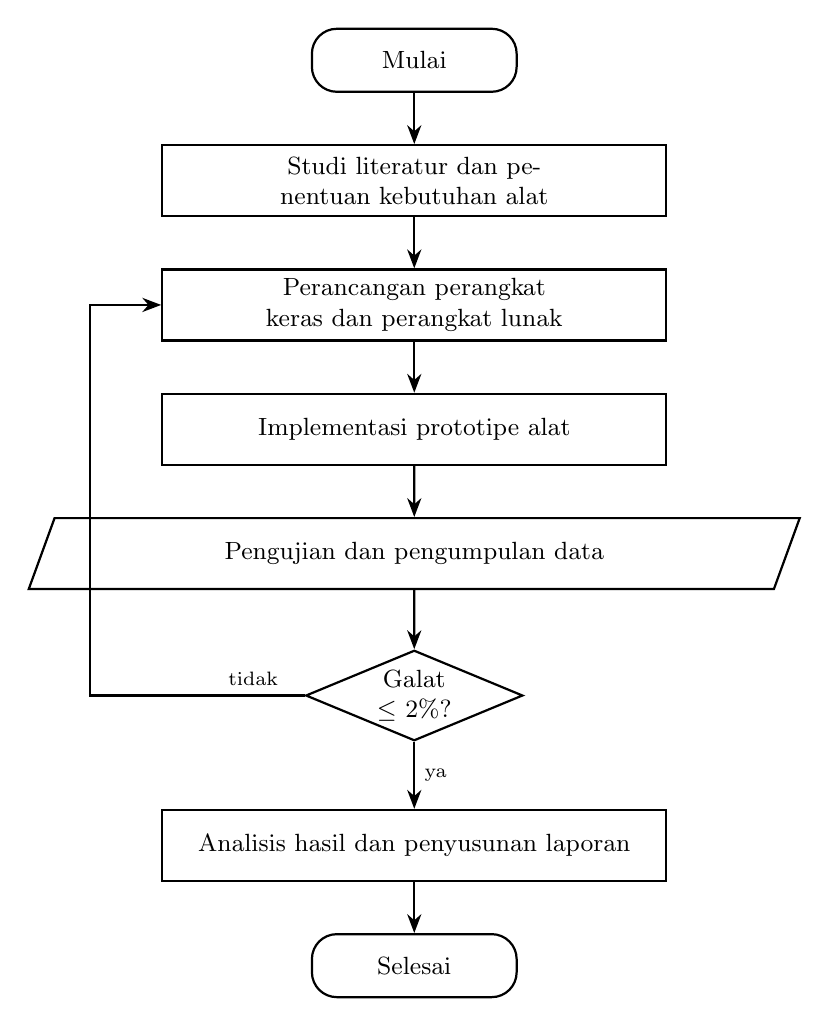
\begin{tikzpicture}[node distance=0.65cm]
\node[term] (a) {Mulai};
\node[proses,below=of a] (b) {Studi literatur dan penentuan kebutuhan alat};
\node[proses,below=of b] (c) {Perancangan perangkat keras dan perangkat lunak};
\node[proses,below=of c] (d) {Implementasi prototipe alat};
\node[io,below=of d] (e) {Pengujian dan pengumpulan data};
\node[putus,below=0.75cm of e] (f) {Galat\\ $\leq$ 2\%?};
\node[proses,below=0.85cm of f] (g) {Analisis hasil dan penyusunan laporan};
\node[term,below=of g] (h) {Selesai};
\foreach \i/\j in {a/b,b/c,c/d,d/e,e/f,g/h} \draw[panah] (\i) -- (\j);
\draw[panah] (f) -- node[right,font=\scriptsize]{ya} (g);
\draw[panah] (f.west) -| node[pos=0.12,above,font=\scriptsize]{tidak} ($(c.west)+(-0.9,0)$) -- (c.west);
\end{tikzpicture}
% ---------- 5. Skema rangkaian ----------
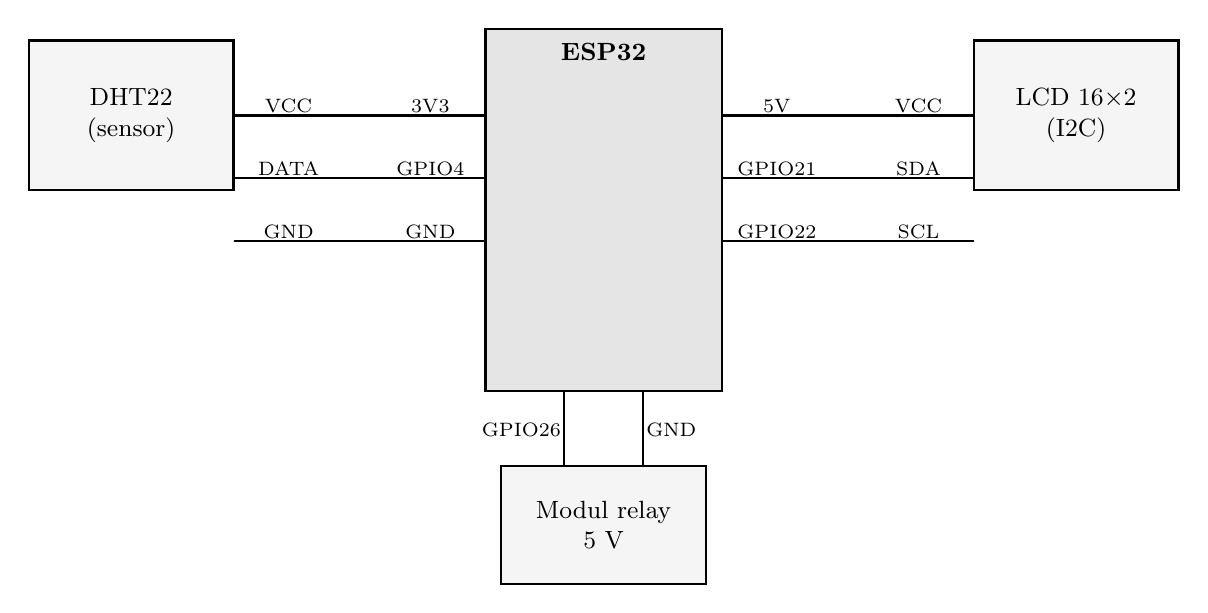
\begin{tikzpicture}
\node[draw,thick,minimum width=3.0cm,minimum height=4.6cm,fill=gray!20] (e) at (0,0) {};
\node[font=\small\bfseries] at (0,2.0) {ESP32};
\node[draw,thick,minimum width=2.6cm,minimum height=1.9cm,fill=gray!8,align=center,font=\small] (s) at (-6.0,1.2) {DHT22\\ (sensor)};
\node[draw,thick,minimum width=2.6cm,minimum height=1.9cm,fill=gray!8,align=center,font=\small] (l) at (6.0,1.2) {LCD 16$\times$2\\ (I2C)};
\node[draw,thick,minimum width=2.6cm,minimum height=1.5cm,fill=gray!8,align=center,font=\small] (r) at (0,-4.0) {Modul relay\\ 5 V};
\foreach \y/\a/\b in {1.2/VCC/3V3,0.4/DATA/GPIO4,-0.4/GND/GND}{
  \draw[thick] (-4.7,\y) -- (-1.5,\y);
  \node[pin,above] at (-4.0,\y) {\a}; \node[pin,above] at (-2.2,\y) {\b};}
\foreach \y/\a/\b in {1.2/VCC/5V,0.4/SDA/GPIO21,-0.4/SCL/GPIO22}{
  \draw[thick] (1.5,\y) -- (4.7,\y);
  \node[pin,above] at (2.2,\y) {\b}; \node[pin,above] at (4.0,\y) {\a};}
\draw[thick] (-0.5,-2.3) -- (-0.5,-3.25); \node[pin,left] at (-0.5,-2.8) {GPIO26};
\draw[thick] (0.5,-2.3) -- (0.5,-3.25); \node[pin,right] at (0.5,-2.8) {GND};
\end{tikzpicture}
% ---------- 6. Prototipe alat tampak depan ----------
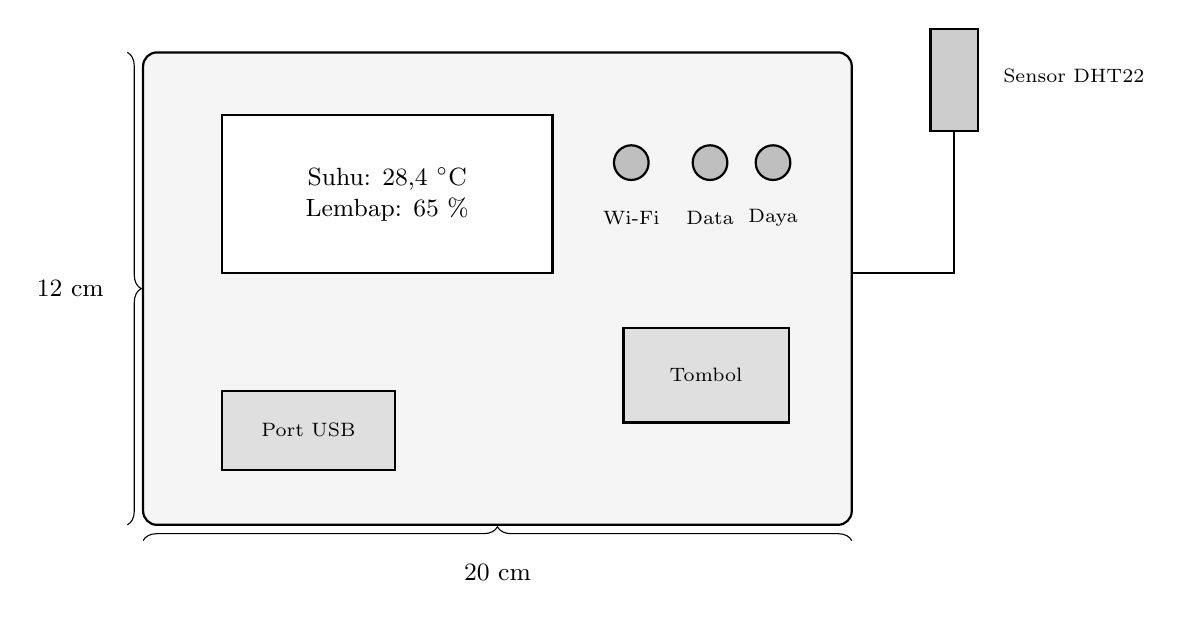
\begin{tikzpicture}
\draw[thick,rounded corners=5pt,fill=gray!8] (0,0) rectangle (9,6);
\draw[thick,fill=white] (1,3.2) rectangle (5.2,5.2); \node[font=\small,align=center] at (3.1,4.2) {Suhu: 28,4 $^\circ$C\\ Lembap: 65 \%};
\foreach \x/\t in {6.2/Wi-Fi,7.2/Data,8.0/Daya}{
  \draw[thick,fill=gray!50] (\x,4.6) circle (0.22); \node[font=\scriptsize] at (\x,3.9) {\t};}
\draw[thick,fill=gray!25] (6.1,1.3) rectangle (8.2,2.5); \node[font=\scriptsize] at (7.15,1.9) {Tombol};
\draw[thick,fill=gray!25] (1.0,0.7) rectangle (3.2,1.7); \node[font=\scriptsize] at (2.1,1.2) {Port USB};
\draw[thick] (9,3.2) -- (10.3,3.2) -- (10.3,5.0); \draw[thick,fill=gray!40] (10.0,5.0) rectangle (10.6,6.3);
\node[font=\scriptsize,anchor=west] at (10.8,5.7) {Sensor DHT22};
\draw[decorate,decoration={brace,amplitude=5pt}] (0,-0.2) -- node[below=5pt,font=\small]{20 cm} (9,-0.2);
\draw[decorate,decoration={brace,mirror,amplitude=5pt}] (-0.2,0) -- node[left=5pt,font=\small]{12 cm} (-0.2,6);
\end{tikzpicture}
\end{document}
